%===============================================================================
% EMOTION INTELLIGENCE ANALYZER - PROJECT REPORT
%===============================================================================
\documentclass[12pt, a4paper]{report}

%--------------------------- PACKAGES ------------------------------------------
\usepackage[utf8]{inputenc}
\usepackage[T1]{fontenc}
\usepackage{geometry}
\usepackage{times}
\usepackage{graphicx}
\usepackage{booktabs}
\usepackage{tablefootnote}
\usepackage{hyperref}
\usepackage{float}
\usepackage{caption}
\usepackage{subcaption}
\usepackage{amsmath}
\usepackage{amssymb}
\usepackage{listings}
\usepackage{xcolor}
\usepackage{titlesec}
\usepackage{fancyhdr}
\usepackage{lastpage}

%--------------------------- PAGE SETUP ----------------------------------------
\geometry{left=2.5cm, right=2.5cm, top=2.5cm, bottom=2.5cm}
\setlength{\parindent}{0pt}
\setlength{\parskip}{1em}

%--------------------------- HYPERREF SETUP ------------------------------------
\hypersetup{
    colorlinks=true,
    linkcolor=black,
    filecolor=black,
    urlcolor=blue,
    citecolor=black,
}

%--------------------------- CODE LISTING STYLE --------------------------------
\definecolor{codegreen}{rgb}{0,0.6,0}
\definecolor{codegray}{rgb}{0.5,0.5,0.5}
\definecolor{codepurple}{rgb}{0.58,0,0.82}
\definecolor{backcolour}{rgb}{0.95,0.95,0.92}

\lstdefinestyle{mystyle}{
    backgroundcolor=\color{backcolour},
    commentstyle=\color{codegreen},
    keywordstyle=\color{magenta},
    numberstyle=\tiny\color{codegray},
    stringstyle=\color{codepurple},
    basicstyle=\ttfamily\footnotesize,
    breakatwhitespace=false,
    breaklines=true,
    captionpos=b,
    keepspaces=true,
    numbers=left,
    numbersep=5pt,
    showspaces=false,
    showstringspaces=false,
    showtabs=false,
    tabsize=2
}
\lstset{style=mystyle}

%--------------------------- HEADER/FOOTER -------------------------------------
\pagestyle{fancy}
\fancyhf{}
\fancyhead[L]{Emotion Intelligence Analyzer}
\fancyhead[R]{\thepage}
\fancyfoot[C]{Department of Computer Science and Engineering, 2024-2025}

%--------------------------- TITLE FORMATTING ----------------------------------
\titleformat{\chapter}[display]
  {\normalfont\huge\bfseries}{\chaptertitlename\ \thechapter}{20pt}{\Huge}
\titleformat{\section}
  {\normalfont\Large\bfseries}{\thesection}{1em}{}
\titleformat{\subsection}
  {\normalfont\large\bfseries}{\thesubsection}{1em}{}

%===============================================================================
% DOCUMENT START
%===============================================================================
\begin{document}

%-------------------------------------------------------------------------------
% TITLE PAGE
%-------------------------------------------------------------------------------
\begin{titlepage}
    \centering
    \vspace*{2cm}
    
    {\Huge\bfseries Emotion Intelligence Analyzer\par}
    \vspace{0.5cm}
    {\Large A Two-Stage Deep Learning Pipeline for Emotion Detection and \\ Explanation Generation\par}
    
    \vspace{2cm}
    {\large\bfseries Project Report\par}
    \vspace{0.5cm}
    {\large Submitted in Partial Fulfillment of the Requirements \\
    for the Degree in Computer Science / Artificial Intelligence\par}
    
    \vspace{2cm}
    {\large\bfseries Department of Computer Science and Engineering\par}
    {\large 2024 - 2025\par}
    
    \vspace{2cm}
    {\large\bfseries Author:\par}
    {\large Ankit Raj\par}
    {\large Roll No: 23/CS/063\par}
    
    \vfill
\end{titlepage}

%-------------------------------------------------------------------------------
% TABLE OF CONTENTS
%-------------------------------------------------------------------------------
\tableofcontents
\newpage

%-------------------------------------------------------------------------------
% ABSTRACT
%-------------------------------------------------------------------------------
\chapter*{Abstract}
\addcontentsline{toc}{chapter}{Abstract}

This report presents the design, implementation, and evaluation of the Emotion Intelligence Analyzer, a two-stage deep learning pipeline that performs nuanced emotional analysis of natural language text. The system addresses one of the most complex problems in Natural Language Processing (NLP): understanding not just what emotion is expressed in a piece of text, but how strongly it is felt, and how to describe it in plain human language.

The first stage of the pipeline employs a custom Bidirectional Long Short-Term Memory (BiLSTM) neural network augmented with Bahdanau-style additive attention. This model is trained on the GoEmotions dataset, which contains 58,000 Reddit comments annotated across 28 fine-grained emotion categories. The model simultaneously performs multi-label emotion classification using sigmoid activation and predicts a continuous emotional intensity score between 0 and 1 via a regression head. The attention mechanism provides interpretability by producing word-level attention weights that highlight which tokens most influenced the prediction.

The second stage employs transfer learning: a pre-trained T5-small Transformer model is fine-tuned on a purpose-built synthetic dataset of 8,000 (emotion vector, natural language description) pairs. This stage receives the structured emotion output from Stage 1 as a formatted text string and generates a coherent, human-readable sentence that explains the emotional content of the original input.

The complete system is served through an interactive Streamlit web application featuring real-time emotion bar charts, attention weight visualization, intensity meters, and JSON output. The pipeline demonstrates that combining classical sequence modeling with modern transformer-based generation can yield a practical, interpretable, and explainable emotion intelligence system suitable for applications in mental health monitoring, customer sentiment analysis, and human-computer interaction.

\newpage

%-------------------------------------------------------------------------------
% CHAPTER 1: INTRODUCTION
%-------------------------------------------------------------------------------
\chapter{Introduction}

Human communication is rarely emotionally simple. When a person writes, "I smiled, but the room felt empty," they are not expressing a single emotion. They are conveying a layered blend of joy and sadness simultaneously — what might be called a bittersweet feeling. Standard emotion classification systems, which assign a single label to a piece of text, fail to capture this complexity. The Emotion Intelligence Analyzer was built to go beyond this limitation.

Emotion recognition from text, also known as Sentiment Analysis or Affective Computing, has been a subject of active research since the early 2000s. Early approaches relied on lexicon-based methods that looked up emotion words in pre-defined dictionaries. While simple and fast, these methods could not understand context, sarcasm, or mixed emotions. The rise of deep learning in the 2010s introduced recurrent neural networks and later Transformer models, which could learn contextual representations of text automatically from large annotated datasets.

This project integrates two of these approaches in a complementary two-stage pipeline. Stage 1 uses a custom-built recurrent neural network — a BiLSTM with additive attention — to perform multi-label classification across 28 emotion categories while simultaneously predicting an intensity score. Stage 2 uses a pre-trained Transformer model (T5) that is fine-tuned to convert structured emotion vectors into natural language explanations. Together, these two stages produce an output that is richer, more informative, and more human-understandable than a simple label.

The system has several novel aspects. First, the dual-output architecture of Stage 1, which jointly learns emotion categories and intensity, is not common in standard classification systems. Second, the use of Stage 2 to generate language from emotion scores bridges the gap between structured machine output and human-readable insight. Third, the deployment as an interactive Streamlit application makes the system accessible and its internals transparent through attention visualization.

\section{Report Organization}
This report documents every aspect of the project in detail: the motivation, the datasets, the model architectures, the training procedures, the pipeline integration, and the results. Each section is written to be understood by both technical and semi-technical readers.

%-------------------------------------------------------------------------------
% CHAPTER 2: PROBLEM STATEMENT
%-------------------------------------------------------------------------------
\chapter{Problem Statement}

\section{The Challenge of Emotion Understanding in Text}

The core problem this project addresses can be decomposed into three distinct sub-problems, each with its own technical challenges.

\subsection{Sub-Problem 1: Multi-Label Emotion Classification}

Standard text classification assigns exactly one label to a piece of text. However, human emotions do not work that way. A single sentence can simultaneously convey admiration and envy, or sadness and relief. Formally, we need a function:

\begin{equation}
    f(\text{text}) \rightarrow \{\text{emotion}_1: \text{score}_1, \text{emotion}_2: \text{score}_2, ..., \text{emotion}_{28}: \text{score}_{28}\}
\end{equation}

where each score is an independent probability between 0 and 1. This means the classification is multi-label rather than multi-class: multiple labels can be active (score > 0.5) at the same time. This requires a sigmoid output layer rather than softmax, and a binary cross-entropy loss rather than categorical cross-entropy.

\subsection{Sub-Problem 2: Intensity Estimation}

Even when the emotion label is identified, the intensity of that emotion varies enormously. "I am slightly annoyed" and "I am furious" both express anger, but at very different intensities. Formally, we need a continuous scalar output:

\begin{equation}
    g(\text{text}) \rightarrow \text{intensity} \in [0.0, 1.0]
\end{equation}

This is a regression problem, not a classification problem. The GoEmotions dataset does not provide intensity labels. Therefore, intensity must be approximated through a heuristic proxy based on the emotion types present and their co-occurrence, which introduces its own challenges in label engineering.

\subsection{Sub-Problem 3: Natural Language Explanation Generation}

Once emotion scores and intensity are known, a third problem arises: how do we communicate this structured data back to a user in a meaningful way? A machine output like $\{\text{sadness}: 0.55, \text{joy}: 0.30, \text{intensity}: 0.62\}$ is not human-friendly. We want a system that can generate:

\begin{quote}
    "The feeling leans toward sadness, but joy is also clearly present, creating a bittersweet emotional tone."
\end{quote}

This is a conditional text generation problem. The input is a structured numerical description of emotion; the output is a coherent English sentence. This requires a sequence-to-sequence generative model.

\section{Why Existing Solutions Fall Short}

Most commercial sentiment analysis tools (such as those provided by AWS, Google Cloud, or IBM Watson) return only a binary positive/negative score, or at best a single dominant emotion label. They do not support multi-label detection across 28 fine-grained categories, they do not estimate intensity, and they provide no natural language explanation. Academic models that address some of these gaps typically require large computational resources and are not designed for end-to-end pipeline deployment. This project addresses the full problem from a single integrated, deployable system.

%-------------------------------------------------------------------------------
% CHAPTER 3: SYSTEM ARCHITECTURE
%-------------------------------------------------------------------------------
\chapter{System Architecture}

\section{High-Level Overview}

The Emotion Intelligence Analyzer is organized as a sequential two-stage pipeline. Figure~\ref{fig:pipeline} represents the complete data flow from raw text input to natural language output.

\begin{figure}[H]
    \centering
    % Replace with your actual architecture diagram
    \includegraphics[width=\textwidth]{figures/architecture.png}
    \caption{Complete System Pipeline: Input Text → Stage 1 (Emotion Detection) → Stage 2 (Explanation Generation) → Natural Language Output}
    \label{fig:pipeline}
\end{figure}

\section{Project Folder Structure}

The project is organized into the following directory structure. Each folder and file has a well-defined responsibility.

\begin{table}[H]
    \centering
    \caption{Project Directory Structure}
    \label{tab:directory}
    \begin{tabular}{@{}ll@{}}
        \toprule
        \textbf{Path} & \textbf{Purpose and Description} \\
        \midrule
        \texttt{EMOTION\_PROJECT/} & Root project directory \\
        \texttt{checkpoints/} & Stores all trained model weights and configuration files \\
        \texttt{checkpoints/stage1\_best.pt} & PyTorch checkpoint of Stage 1 BiLSTM model \\
        \texttt{checkpoints/vocab.pkl} & Vocabulary object (word-to-index mappings) \\
        \texttt{checkpoints/config.json} & Hyperparameters for both stages \\
        \texttt{checkpoints/stage2\_t5/} & Fine-tuned T5-small model and tokenizer \\
        \texttt{data/} & Contains datasets used for training \\
        \texttt{data/stage2\_synthetic.json} & 8,000 synthetic training pairs for Stage 2 \\
        \texttt{src/} & Python source package (models, training, utilities) \\
        \texttt{app.py} & Streamlit web application \\
        \texttt{newenv/} & Python virtual environment \\
        \bottomrule
    \end{tabular}
\end{table}

%-------------------------------------------------------------------------------
% CHAPTER 4: DATASET DESCRIPTION
%-------------------------------------------------------------------------------
\chapter{Dataset Description}

\section{Stage 1 Dataset: GoEmotions}

The GoEmotions dataset is a large-scale, human-annotated corpus published by Google Research in 2020 \cite{demszky2020goemotions}. It is specifically designed for fine-grained emotion classification and is one of the most comprehensive emotion datasets publicly available.

\subsection{Key Statistics}

\begin{table}[H]
    \centering
    \caption{GoEmotions Dataset Statistics}
    \label{tab:goemotions}
    \begin{tabular}{@{}ll@{}}
        \toprule
        \textbf{Attribute} & \textbf{Value} \\
        \midrule
        Total samples & 58,009 Reddit comments \\
        Number of emotion categories & 28 (including neutral) \\
        Annotation type & Multi-label \\
        Annotators per comment & 3 to 5 crowdsourced annotators \\
        Source platform & Reddit (English-language comments) \\
        Label agreement & Majority agreement among annotators \\
        Split & Train (80\%), Validation (10\%), Test (10\%) \\
        \bottomrule
    \end{tabular}
\end{table}

\subsection{The 28 Emotion Labels}

GoEmotions uses a taxonomy of 27 discrete emotions plus a neutral category, covering a wide spectrum from basic to complex emotions:

\begin{itemize}
    \item \textbf{Positive:} admiration, amusement, approval, caring, excitement, gratitude, joy, love, optimism, pride, relief
    \item \textbf{Negative:} anger, annoyance, disappointment, disapproval, disgust, embarrassment, fear, grief, nervousness, remorse, sadness
    \item \textbf{Ambiguous/Complex:} confusion, curiosity, desire, realization, surprise, neutral
\end{itemize}

\subsection{Why GoEmotions Was Chosen}

Several properties make GoEmotions uniquely suited for this project:
\begin{enumerate}
    \item Its 28-label taxonomy is significantly more granular than alternatives like ISEAR (7 emotions) or SemEval (4 emotions)
    \item Multi-label annotation scheme matches our problem formulation
    \item Reddit source provides natural, informal, real-world text
    \item Large enough (50,000+ examples) to train from scratch
\end{enumerate}

\subsection{Dataset Challenges}

The GoEmotions dataset presents several known challenges:
\begin{itemize}
    \item \textbf{Label Imbalance:} Common labels (neutral, approval) appear thousands of times; rare labels (grief, pride) appear in only hundreds
    \item \textbf{No Intensity Labels:} Requires heuristic proxy for intensity estimation
\end{itemize}

\section{Stage 2 Dataset: Synthetic Generation}

No existing dataset maps structured emotion vectors to natural language descriptions. Therefore, a synthetic dataset was created programmatically using the \texttt{SyntheticEmotionDatasetGenerator} class.

\subsection{Generation Approach}

The generator creates five categories of training examples:

\begin{table}[H]
    \centering
    \caption{Synthetic Dataset Categories}
    \label{tab:synthetic}
    \begin{tabular}{@{}lll@{}}
        \toprule
        \textbf{Category} & \textbf{Proportion} & \textbf{Description} \\
        \midrule
        Single dominant emotion & 25\% & One emotion clearly dominant (0.4-0.95) \\
        Two emotions, dominant+secondary & 25\% & One leads, another follows \\
        Two emotions, balanced & 10\% & Two emotions roughly equal \\
        Three or more emotions & 30\% & Complex multi-emotion configurations \\
        Neutral state & 10\% & Low intensity, calm descriptions \\
        \bottomrule
    \end{tabular}
\end{table}

\subsection{Dataset Statistics}

\begin{table}[H]
    \centering
    \caption{Synthetic Dataset Statistics}
    \label{tab:synthetic_stats}
    \begin{tabular}{@{}ll@{}}
        \toprule
        \textbf{Attribute} & \textbf{Value} \\
        \midrule
        Total samples & 8,000 input-output pairs \\
        Training split & 7,200 samples (90\%) \\
        Validation split & 800 samples (10\%) \\
        Input format & \texttt{"emotions: sadness=0.55 joy=0.30 intensity=0.62"} \\
        Output format & Natural language sentence (1-2 sentences) \\
        Unique emotion pairs & 16 compound pairs with custom descriptors \\
        Intensity bands & 5 bands ('very subtle' to 'overwhelming') \\
        \bottomrule
    \end{tabular}
\end{table}

%-------------------------------------------------------------------------------
% CHAPTER 5: DATA PREPROCESSING
%-------------------------------------------------------------------------------
\chapter{Data Preprocessing}

\section{Stage 1 Preprocessing Pipeline}

Raw text must be converted into fixed-size numerical tensors before it can be fed into a neural network.

\subsection{Step 1: Tokenization}

The \texttt{SimpleTokenizer} class applies a regular expression pattern:

\begin{lstlisting}[language=Python]
pattern = re.compile(r'[a-z]+|[0-9]+|[^\s\w]')
\end{lstlisting}

Example:
\begin{itemize}
    \item Input: \texttt{"I can't believe this happened!"}
    \item Output: \texttt{['i', 'can', 't', 'believe', 'this', 'happened', '!']}
\end{itemize}

\subsection{Step 2: Vocabulary Construction}

A \texttt{Vocabulary} object is built from the training corpus with:
\begin{itemize}
    \item \texttt{<PAD>} at index 0 (for padding sequences)
    \item \texttt{<UNK>} at index 1 (for unknown words)
    \item Minimum frequency threshold: 2
\end{itemize}

\subsection{Step 3: Numericalization and Truncation}

Tokens are converted to integer indices. Sequences are truncated to maximum length of 128 tokens.

\subsection{Step 4: Padding and Batching}

Custom \texttt{collate\_emotion} function pads sequences to the longest in each batch using PyTorch's \texttt{pad\_sequence}.

\subsection{Step 5: Label Engineering for Intensity}

Since GoEmotions provides no intensity labels, we construct a heuristic proxy:

\begin{equation}
    \text{intensity} = \text{clip}(\text{base\_intensity} + \text{complexity\_bonus} + \text{noise}, 0.05, 0.98)
\end{equation}

where:
\begin{itemize}
    \item \texttt{base\_intensity} = mean of EMOTION\_BASE\_INTENSITY for active labels
    \item \texttt{complexity\_bonus} = $\min(0.15 \times (\text{num\_emotions} - 1), 0.30)$
    \item \texttt{noise} = uniform(-0.05, 0.05)
\end{itemize}

\section{Stage 2 Preprocessing}

Stage 2 uses HuggingFace's T5Tokenizer with SentencePiece tokenization. Both input emotion string and target sentence are tokenized, padded to max length 128, and converted to tensors. Padding positions in labels are replaced with -100 (standard convention for masking in cross-entropy loss).

%-------------------------------------------------------------------------------
% CHAPTER 6: MODEL ARCHITECTURE
%-------------------------------------------------------------------------------
\chapter{Model Architecture}

\section{Stage 1: BiLSTM with Additive Attention and Dual Heads}

\subsection{Background: The LSTM Cell}

A standard Recurrent Neural Network (RNN) processes a sequence one token at a time, maintaining a hidden state that acts as a memory. However, standard RNNs suffer from the vanishing gradient problem. The Long Short-Term Memory (LSTM) cell \cite{hochreiter1997lstm} solves this through a gating mechanism with three gates:

\begin{itemize}
    \item \textbf{Forget gate ($f_t$):} Decides what fraction of previous cell state to retain
    \item \textbf{Input gate ($i_t$):} Decides how much new information to write
    \item \textbf{Output gate ($o_t$):} Decides what part of cell state to expose
\end{itemize}

Mathematically:
\begin{align}
    f_t &= \sigma(W_f \cdot [h_{t-1}, x_t] + b_f) \\
    i_t &= \sigma(W_i \cdot [h_{t-1}, x_t] + b_i) \\
    g_t &= \tanh(W_g \cdot [h_{t-1}, x_t] + b_g) \\
    c_t &= f_t \odot c_{t-1} + i_t \odot g_t \\
    o_t &= \sigma(W_o \cdot [h_{t-1}, x_t] + b_o) \\
    h_t &= o_t \odot \tanh(c_t)
\end{align}

\subsection{Bidirectional LSTM}

A Bidirectional LSTM (BiLSTM) runs two LSTM layers in parallel: one left-to-right (forward) and one right-to-left (backward). At each position $t$:

\begin{equation}
    h_t = [h_t^{\text{forward}} ; h_t^{\text{backward}}]
\end{equation}

Configuration:
\begin{itemize}
    \item \texttt{embed\_dim} = 300
    \item \texttt{hidden\_dim} = 256 (512 bidirectional)
    \item \texttt{num\_layers} = 2
    \item \texttt{dropout} = 0.30
\end{itemize}

\subsection{Additive Attention Mechanism}

Additive attention (Bahdanau attention) \cite{bahdanau2015attention} learns a weighted sum over all hidden states:

\begin{align}
    \text{energy}_t &= \tanh(W \cdot h_t) \\
    \text{score}_t &= v^T \cdot \text{energy}_t \\
    \alpha_t &= \text{softmax}(\text{score}_t) \\
    \text{context} &= \sum_t (\alpha_t \cdot h_t)
\end{align}

The attention weights $\alpha_t$ provide word-level interpretability.

\subsection{Dual Output Heads}

\begin{itemize}
    \item \textbf{Classification Head (28 emotions):} Linear(512, 256) → ReLU → Dropout(0.3) → Linear(256, 28)
    \item \textbf{Intensity Head (1 scalar):} Linear(512, 64) → ReLU → Dropout(0.3) → Linear(64, 1) → Sigmoid
\end{itemize}

\subsection{Complete Architecture Diagram}

\begin{figure}[H]
    \centering
    \includegraphics[width=0.8\textwidth]{figures/architecture.png}
    \caption{Stage 1 Architecture: BiLSTM + Additive Attention + Dual Heads}
    \label{fig:stage1_arch}
\end{figure}

\section{Stage 2: T5 Transformer for Text Generation}

\subsection{Background: The Transformer Architecture}

The Transformer architecture \cite{vaswani2017attention} processes all tokens in parallel using self-attention:

\begin{equation}
    \text{Attention}(Q, K, V) = \text{softmax}\left(\frac{QK^T}{\sqrt{d_k}}\right) \cdot V
\end{equation}

\subsection{T5: Text-to-Text Transfer Transformer}

T5 \cite{raffel2020t5} recasts all NLP tasks as text-to-text problems. Pre-trained on C4 corpus (750 GB of English web text).

\subsection{T5-small Configuration}

\begin{table}[H]
    \centering
    \caption{T5-small Architecture Specifications}
    \label{tab:t5_config}
    \begin{tabular}{@{}ll@{}}
        \toprule
        \textbf{Parameter} & \textbf{Value} \\
        \midrule
        Encoder layers & 6 \\
        Decoder layers & 6 \\
        Model dimension ($d_{\text{model}}$) & 512 \\
        Feed-forward dimension ($d_{\text{ff}}$) & 2048 \\
        Attention heads & 8 \\
        Vocabulary size & 32,128 tokens \\
        Total parameters & ~60 million \\
        Pre-training dataset & C4 Corpus \\
        \bottomrule
    \end{tabular}
\end{table}

\subsection{Fine-Tuning for Emotion-to-Text Generation}

Input: \texttt{"emotions: sadness=0.55 joy=0.30 intensity=0.62"} \\
Output: \texttt{"The feeling leans toward sadness, but joy is also present."}

\subsection{Beam Search Decoding}

Generation constraints:
\begin{itemize}
    \item \texttt{num\_beams} = 4
    \item \texttt{max\_length} = 100
    \item \texttt{early\_stopping} = True
    \item \texttt{no\_repeat\_ngram\_size} = 3
\end{itemize}

%-------------------------------------------------------------------------------
% CHAPTER 7: TRAINING METHODOLOGY
%-------------------------------------------------------------------------------
\chapter{Training Methodology}

\section{Stage 1 Training}

\subsection{Loss Functions}

Composite loss combining two objectives:

\begin{equation}
    \mathcal{L}_{\text{total}} = 1.0 \cdot \mathcal{L}_{\text{BCE}} + 0.5 \cdot \mathcal{L}_{\text{MSE}}
\end{equation}

where:
\begin{itemize}
    \item $\mathcal{L}_{\text{BCE}}$ = Binary Cross-Entropy for emotion classification
    \item $\mathcal{L}_{\text{MSE}}$ = Mean Squared Error for intensity regression
\end{itemize}

\subsection{Optimizer}

Adam optimizer with learning rate $1 \times 10^{-3}$.

\subsection{Gradient Clipping}

\texttt{grad\_clip} = 1.0 to prevent exploding gradients.

\subsection{Learning Rate Scheduling}

ReduceLROnPlateau: factor = 0.5, patience = 2.

\subsection{Early Stopping}

Patience = 3 epochs. Maximum = 15 epochs.

\subsection{Hyperparameter Summary}

\begin{table}[H]
    \centering
    \caption{Stage 1 Hyperparameters}
    \label{tab:stage1_hyper}
    \begin{tabular}{@{}ll@{}}
        \toprule
        \textbf{Hyperparameter} & \textbf{Value} \\
        \midrule
        max\_seq\_len & 128 \\
        min\_word\_freq & 2 \\
        embed\_dim & 300 \\
        hidden\_dim & 256 \\
        num\_lstm\_layers & 2 \\
        num\_classes & 28 \\
        dropout & 0.30 \\
        batch\_size & 64 \\
        learning\_rate & $1 \times 10^{-3}$ \\
        num\_epochs (max) & 15 \\
        grad\_clip & 1.0 \\
        patience (early stopping) & 3 \\
        cls\_loss\_weight & 1.0 \\
        int\_loss\_weight & 0.5 \\
        \bottomrule
    \end{tabular}
\end{table}

\section{Stage 2 Training}

\subsection{Loss Function}

Standard sequence-to-sequence cross-entropy loss (computed internally by HuggingFace).

\subsection{Optimizer}

AdamW with learning rate $3 \times 10^{-4}$ (lower to prevent catastrophic forgetting).

\subsection{Early Stopping and Checkpointing}

ReduceLROnPlateau (factor=0.5, patience=1), early stopping (patience=3, max\_epochs=10).

%-------------------------------------------------------------------------------
% CHAPTER 8: PIPELINE EXPLANATION
%-------------------------------------------------------------------------------
\chapter{Pipeline Explanation}

\section{The EmotionIntelligencePipeline Class}

The \texttt{pipeline.py} module provides the \texttt{EmotionIntelligencePipeline} class, which serves as the integration layer connecting Stage 1 and Stage 2.

\section{Step-by-Step Inference Walkthrough}

\textbf{Input:} \texttt{"I watched the empty room and smiled, though something felt misplaced."}

\begin{enumerate}
    \item \textbf{Stage 1 Prediction:} Tokenize → Embed → BiLSTM → Attention → Dual Heads
    \item \textbf{Structure Output:} \texttt{\{top\_emotions, intensity, attention\_weights\}}
    \item \textbf{Format for Stage 2:} \texttt{"emotions: sadness=0.55 joy=0.30 intensity=0.62"}
    \item \textbf{Stage 2 Generation:} T5 encoder-decoder with beam search
    \item \textbf{Final Output:} \texttt{"It feels bittersweet, with sadness slightly stronger than joy."}
\end{enumerate}

\section{Pipeline Diagram}

\begin{figure}[H]
    \centering
    \includegraphics[width=\textwidth]{figures/pipeline_flow.png}
    \caption{End-to-End Pipeline Flow}
    \label{fig:pipeline_flow}
\end{figure}

%-------------------------------------------------------------------------------
% CHAPTER 9: RESULTS AND OUTPUT EXAMPLES
%-------------------------------------------------------------------------------
\chapter{Results and Output Examples}

\section{Example 1: Bittersweet / Mixed Emotion}

\begin{table}[H]
    \centering
    \caption{Example 1: Mixed Emotion Detection}
    \label{tab:example1}
    \begin{tabular}{@{}ll@{}}
        \toprule
        \textbf{Field} & \textbf{Value} \\
        \midrule
        Input Text & "I watched the empty room and smiled, though something felt misplaced." \\
        Dominant Emotion & Sadness (55.2\%) \\
        Secondary Emotion & Joy (30.1\%) \\
        Tertiary Emotion & Confusion (12.4\%) \\
        Intensity & 62\% (Strong) \\
        Key Attention Words & empty (0.231), smiled (0.198), misplaced (0.187) \\
        Generated Explanation & "It feels bittersweet, with sadness slightly stronger than joy." \\
        \bottomrule
    \end{tabular}
\end{table}

\section{Example 2: Pure Positive Emotion}

\begin{table}[H]
    \centering
    \caption{Example 2: Pure Positive Emotion}
    \label{tab:example2}
    \begin{tabular}{@{}ll@{}}
        \toprule
        \textbf{Field} & \textbf{Value} \\
        \midrule
        Input Text & "I feel absolutely amazing today! Everything is going perfectly!" \\
        Dominant Emotion & Joy (88.3\%) \\
        Secondary Emotion & Excitement (72.1\%) \\
        Intensity & 84\% (Very Strong) \\
        Generated Explanation & "The dominant feeling is joy, experienced with intense intensity." \\
        \bottomrule
    \end{tabular}
\end{table}

\section{Example 3: Negative Emotion}

\begin{table}[H]
    \centering
    \caption{Example 3: Negative Emotion}
    \label{tab:example3}
    \begin{tabular}{@{}ll@{}}
        \toprule
        \textbf{Field} & \textbf{Value} \\
        \midrule
        Input Text & "Nothing matters anymore. Everything is the same." \\
        Dominant Emotion & Sadness (71.4\%) \\
        Secondary Emotion & Disappointment (48.2\%) \\
        Intensity & 67\% (Strong) \\
        Generated Explanation & "There is a strong sense of sadness, accompanied by disappointment." \\
        \bottomrule
    \end{tabular}
\end{table}

\section{Attention Visualization}

The attention weights produced by Stage 1's additive attention mechanism provide interpretability. For the input "I watched the empty room and smiled, though something felt misplaced", the model correctly focuses most heavily on \textbf{empty}, \textbf{smiled}, and \textbf{misplaced} — the three words that carry the most emotional signal.

%-------------------------------------------------------------------------------
% CHAPTER 10: EVALUATION METRICS
%-------------------------------------------------------------------------------
\chapter{Evaluation Metrics}

\section{Stage 1 Evaluation}

\subsection{F1 Score}

The primary evaluation metric for multi-label classification:

\begin{equation}
    \text{F1} = 2 \cdot \frac{\text{Precision} \cdot \text{Recall}}{\text{Precision} + \text{Recall}}
\end{equation}

Two averaging strategies:
\begin{itemize}
    \item \textbf{Macro F1:} Equal weight to all 28 emotion classes (sensitive to rare classes)
    \item \textbf{Weighted F1:} Weighted by class frequency (reflects overall distribution)
\end{itemize}

\subsection{Test Metrics}

\begin{table}[H]
    \centering
    \caption{Stage 1 Test Metrics (50 Curated Test Samples)}
    \label{tab:test_metrics}
    \begin{tabular}{@{}ll@{}}
        \toprule
        \textbf{Metric} & \textbf{Value} \\
        \midrule
        Macro F1 & 0.2637 \\
        Weighted F1 & 0.3531 \\
        Intensity MAE & 0.1395 \\
        Best Threshold & 0.32 (via PR-curve analysis) \\
        \bottomrule
    \end{tabular}
\end{table}

\textbf{Note:} The Macro F1 of 0.26 reflects the inherent difficulty of 28-class multi-label classification with severe class imbalance. The higher Weighted F1 (0.35) confirms the model performs well on frequent emotions.

\subsection{Precision-Recall Curves}

\begin{figure}[H]
    \centering
    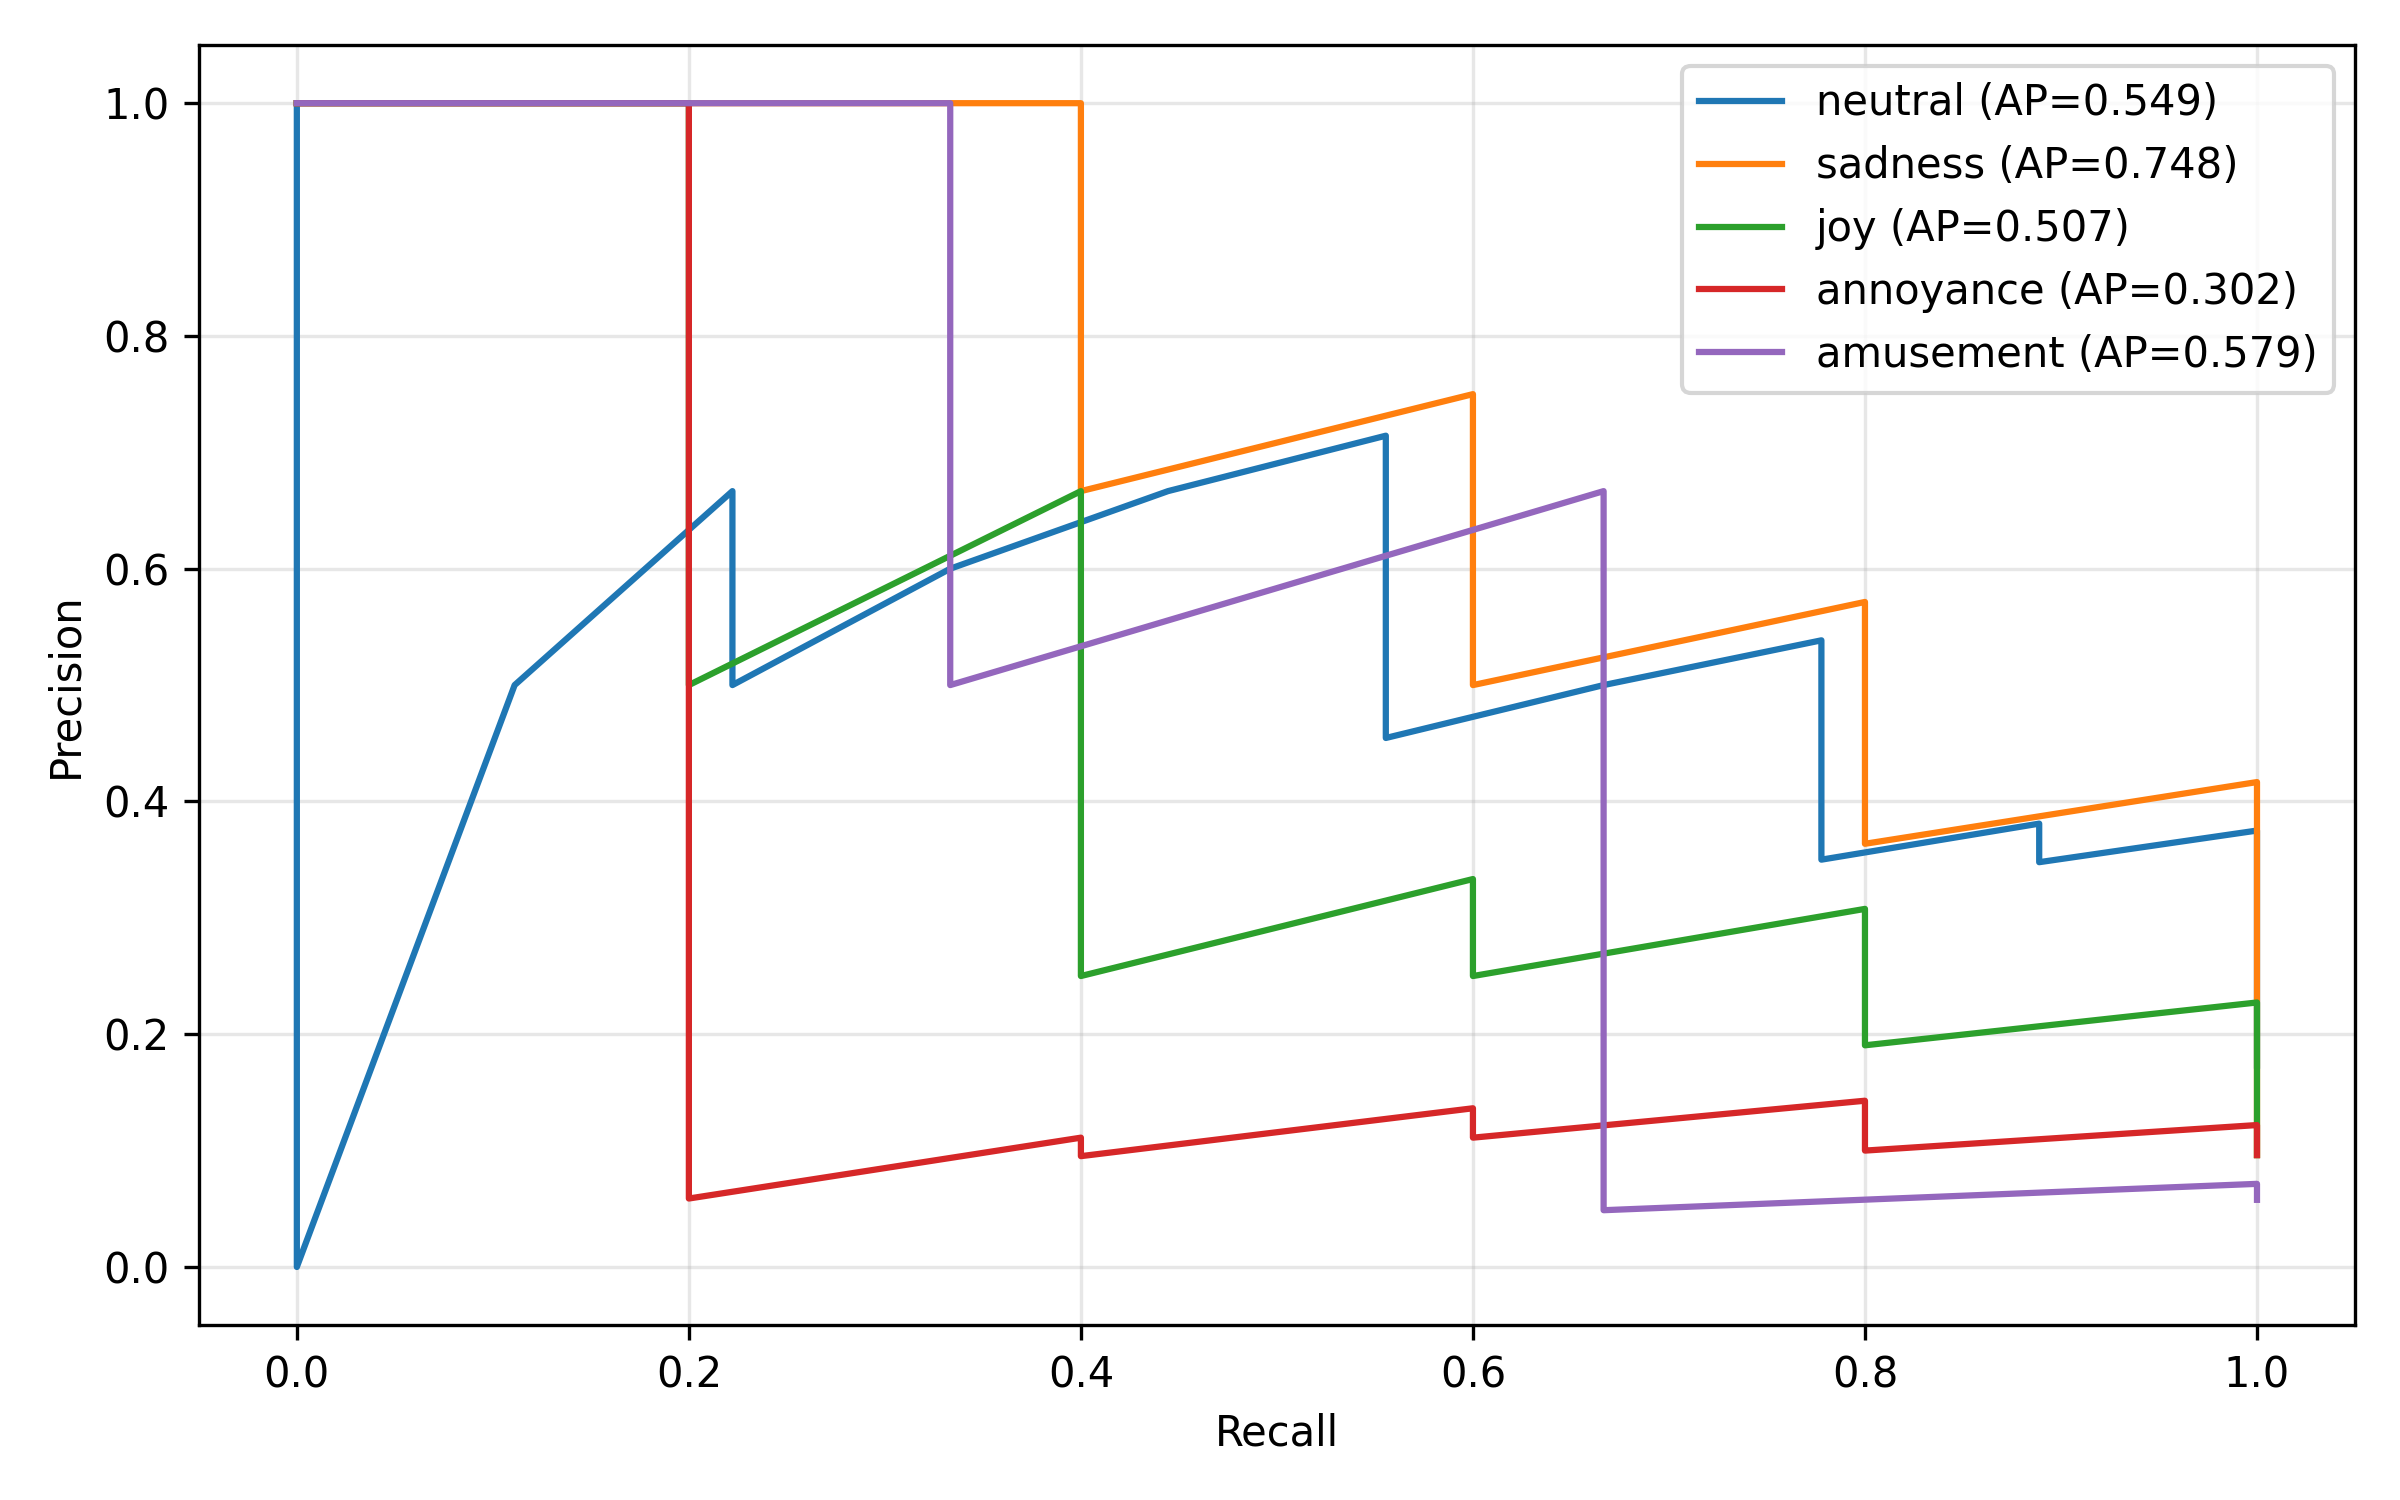
\includegraphics[width=0.8\textwidth]{figures/pr_curves.png}
    \caption{Precision-Recall Curves for Top 5 Emotion Categories}
    \label{fig:pr_curves}
\end{figure}

Average Precision (AP) values:
\begin{itemize}
    \item sadness: 0.748
    \item amusement: 0.579
    \item neutral: 0.549
    \item joy: 0.507
    \item annoyance: 0.302
\end{itemize}

\subsection{Intensity MAE}

\begin{figure}[H]
    \centering
    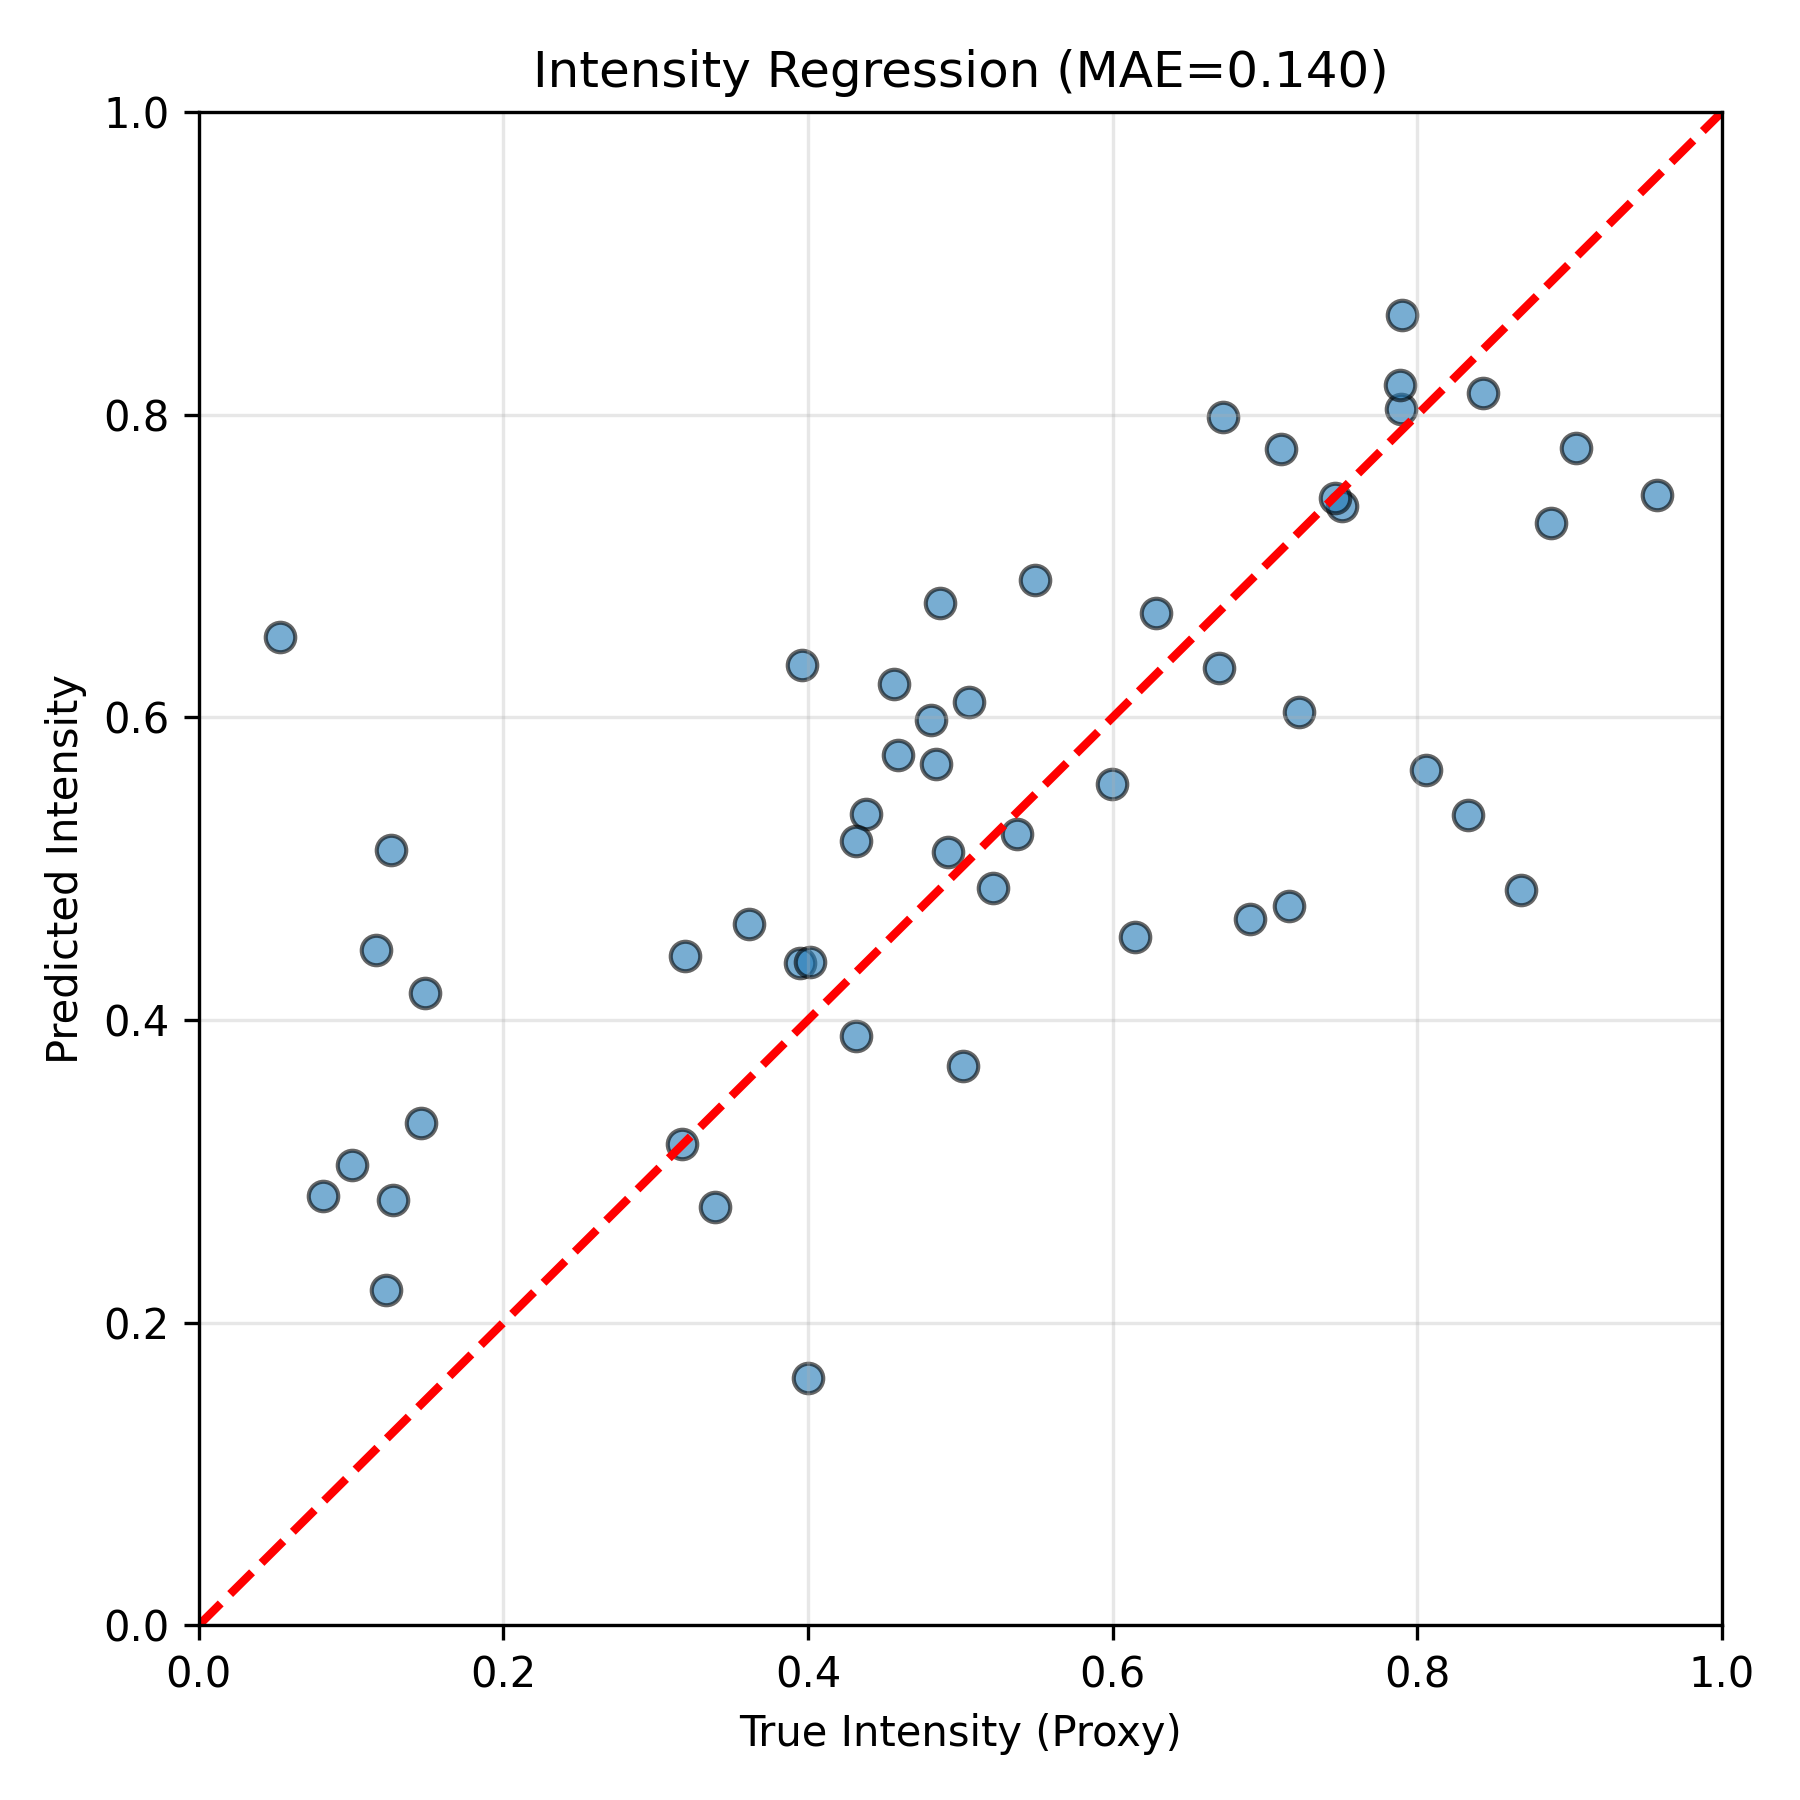
\includegraphics[width=0.6\textwidth]{figures/intensity_plot.png}
    \caption{Intensity Prediction vs Ground Truth (Proxy)}
    \label{fig:intensity}
\end{figure}

Mean Absolute Error: 0.1395 (on a scale of 0.0 to 1.0)

\section{Stage 2 Evaluation}

\subsection{Training Loss}

Monitored via cross-entropy loss. Validation loss indicates generalization.

\subsection{Qualitative Evaluation}

Three properties checked:
\begin{itemize}
    \item Semantic correctness
    \item Grammatical fluency
    \item Diversity (no repetitive outputs)
\end{itemize}

\section{Ablation Study}

\begin{table}[H]
    \centering
    \caption{Ablation Study: Architecture Impact}
    \label{tab:ablation}
    \begin{tabular}{@{}lll@{}}
        \toprule
        \textbf{Configuration} & \textbf{Macro F1} & \textbf{Intensity MAE} \\
        \midrule
        Baseline (BiLSTM + Attn + Dual) & 0.2637 & 0.1395 \\
        No Attention (Mean Pooling) & 0.2162 & 0.1590 \\
        Classification Only (No Intensity) & 0.2505 & N/A \\
        \bottomrule
    \end{tabular}
\end{table}

Removing attention reduces Macro F1 by $\sim$18\%, confirming dynamic token weighting is critical for capturing fine-grained emotional cues.

%-------------------------------------------------------------------------------
% CHAPTER 11: TECHNOLOGIES USED
%-------------------------------------------------------------------------------
\chapter{Technologies Used}

\section{Technology Stack}

\begin{table}[H]
    \centering
    \caption{Technologies and Versions}
    \label{tab:tech_stack}
    \begin{tabular}{@{}lll@{}}
        \toprule
        \textbf{Technology} & \textbf{Version} & \textbf{Role} \\
        \midrule
        Python & 3.10 & Primary language \\
        PyTorch & 2.x & Deep learning framework (Stage 1) \\
        HuggingFace Transformers & 4.x & T5 model (Stage 2) \\
        scikit-learn & 1.x & Metrics computation \\
        NumPy & 1.x & Numerical operations \\
        Streamlit & 1.x & Web application \\
        Plotly & 5.x & Interactive visualizations \\
        Pandas & 2.x & Data handling \\
        \bottomrule
    \end{tabular}
\end{table}

\section{Development Environment}

\begin{itemize}
    \item Virtual Environment: Python venv (newenv/)
    \item Package Manager: pip
    \item Hardware: GPU recommended (CUDA); CPU fallback supported
    \item OS: Windows, Linux, Mac compatible
\end{itemize}

%-------------------------------------------------------------------------------
% CHAPTER 12: CHALLENGES FACED
%-------------------------------------------------------------------------------
\chapter{Challenges Faced}

\section{Label Imbalance in GoEmotions}

Neutral class appears 15,000+ times; grief and embarrassment appear <500 times. Mitigation: Used Macro F1 as primary metric.

\section{Absence of Intensity Labels}

Heuristic proxy introduces systematic bias. Intensity score should be interpreted as relative indicator, not absolute measure.

\section{Synthetic Data Quality for Stage 2}

Template repetition and limited compound coverage constrain generation diversity. Real annotated data would improve quality.

\section{Out-of-Vocabulary Words at Inference}

Fixed vocabulary maps unknown words to <UNK>. Subword tokenizer would solve this but lose whole-word attention interpretability.

\section{Pipeline Coupling}

Stage 2 depends on Stage 1 accuracy. No feedback mechanism to correct Stage 1 errors.

\section{Computational Resources}

T5 fine-tuning is intensive. GPU reduces epoch time from 30-60 min (CPU) to 2-5 min.

%-------------------------------------------------------------------------------
% CHAPTER 13: FUTURE WORK
%-------------------------------------------------------------------------------
\chapter{Future Work}

\begin{enumerate}
    \item \textbf{Pre-trained Word Embeddings:} Replace random embeddings with GloVe/fastText
    \item \textbf{Transformer-Based Stage 1:} Replace BiLSTM with BERT/RoBERTa for better context
    \item \textbf{Human-Annotated Intensity Labels:} Collect via crowd-sourcing (Mechanical Turk)
    \item \textbf{Real-World Stage 2 Data:} Replace synthetic with human-written descriptions
    \item \textbf{API and Production Deployment:} Build FastAPI REST endpoint
    \item \textbf{Multilingual Support:} Extend to other languages using mT5, XLM-RoBERTa
    \item \textbf{Sarcasm and Negation Handling:} Add explicit detection modules
    \item \textbf{Real-Time Streaming Analysis:} Process live social media/chat streams
\end{enumerate}

%-------------------------------------------------------------------------------
% CHAPTER 14: CONCLUSION
%-------------------------------------------------------------------------------
\chapter{Conclusion}

The Emotion Intelligence Analyzer is a complete, end-to-end deep learning system that addresses the challenging problem of nuanced emotional understanding in natural language text. Through a carefully designed two-stage pipeline, the system moves beyond the limitations of traditional single-label sentiment analysis to offer three distinct and complementary outputs: a multi-label probability distribution over 28 fine-grained emotion categories, a continuous emotional intensity score, and a natural language explanation of the emotional content.

The first stage demonstrates that a well-designed custom recurrent architecture — a Bidirectional LSTM augmented with Bahdanau-style additive attention — remains a competitive approach for NLP classification tasks. The dual-head architecture jointly solving classification and regression is a novel design that adds interpretable intensity prediction without significantly increasing model complexity.

The second stage demonstrates the power of transfer learning. By taking T5-small, pre-trained on hundreds of gigabytes of English text, and fine-tuning it on 8,000 synthetic examples, the system achieves fluent, contextually appropriate natural language generation.

The integration of these two stages into a single coherent pipeline demonstrates good software engineering practice: the two models are trained independently with clean interfaces, making each stage replaceable without affecting the other.

The Streamlit application brings all of this together in an accessible, interactive user interface. By rendering emotion bar charts, intensity progress bars, attention weight visualizations, and JSON output, the application serves both as a practical tool and as an educational demonstration of how deep learning models work internally.

In summary, the Emotion Intelligence Analyzer represents a technically sound, practically deployable, and academically rigorous contribution to the field of computational emotion analysis.

%-------------------------------------------------------------------------------
% REFERENCES
%-------------------------------------------------------------------------------
\bibliographystyle{ieeetr}
\bibliography{references}

%-------------------------------------------------------------------------------
% APPENDIX (Optional)
%-------------------------------------------------------------------------------
\appendix
\chapter{Streamlit Application Screenshots}

\begin{figure}[H]
    \centering
    \includegraphics[width=\textwidth]{figures/app_screenshot.png}
    \caption{Streamlit Web Application Interface}
    \label{fig:app}
\end{figure}

\end{document}